\section{Current Practice and Needs}
To learn about current practice and unsupported needs in presentation technology, we conducted multiple rounds of interviews with classroom lecturers, online lecturers, graduate student TAs, and undergraduate students, with varied experiences in giving and listening to presentations. 
%
We also consulted existing literature comparing different types of presentation software.
%
From this analysis, we summarize the key findings that informed the design of our system.

\textbf{Flexibility in presentations is preferred for interactive or informal settings.} For settings such as research conferences or business meetings with tight time constraints and little room for audience interaction, people prefer to give highly scripted presentations with electronic slides. However, for settings such as lectures, tutoring sessions, or brainstorming meetings, presenters like to have some flexibility and often use inking as part of their presentations. Common strategies include using a blackboard or projecting slides/transparencies onto a board and inking on top of them. Several lecturers purposefully leave blank spaces on their slides to fill in by inking during the lecture. %Inking allows presenters to draw attention to content by writing or annotating in real time, to modify the order in which content is presented, or in some cases, to modify the content itself based on audience input or feedback.

\textbf{Presenters want flexibility over prepared contents rather than complete improvisation.} Even for informal settings, presenters have the bulk of the content planned and prepared beforehand, in the form of lecture notes, worksheets or slides. Thus, the type of flexibility that presenters want is the ability to make small-scale adjustments on-the-fly, such as omitting part of the content, adding minor changes such as a line of text or annotations, or changing the order of the contents. Inking is often used to this effect. 
%\wil{This is repetitive with the last sentence in the previous paragraph.}
\begin{figure*}[ht!]
    \centering
    \begin{subfigure}[t]{0.32\textwidth}
        \centering
        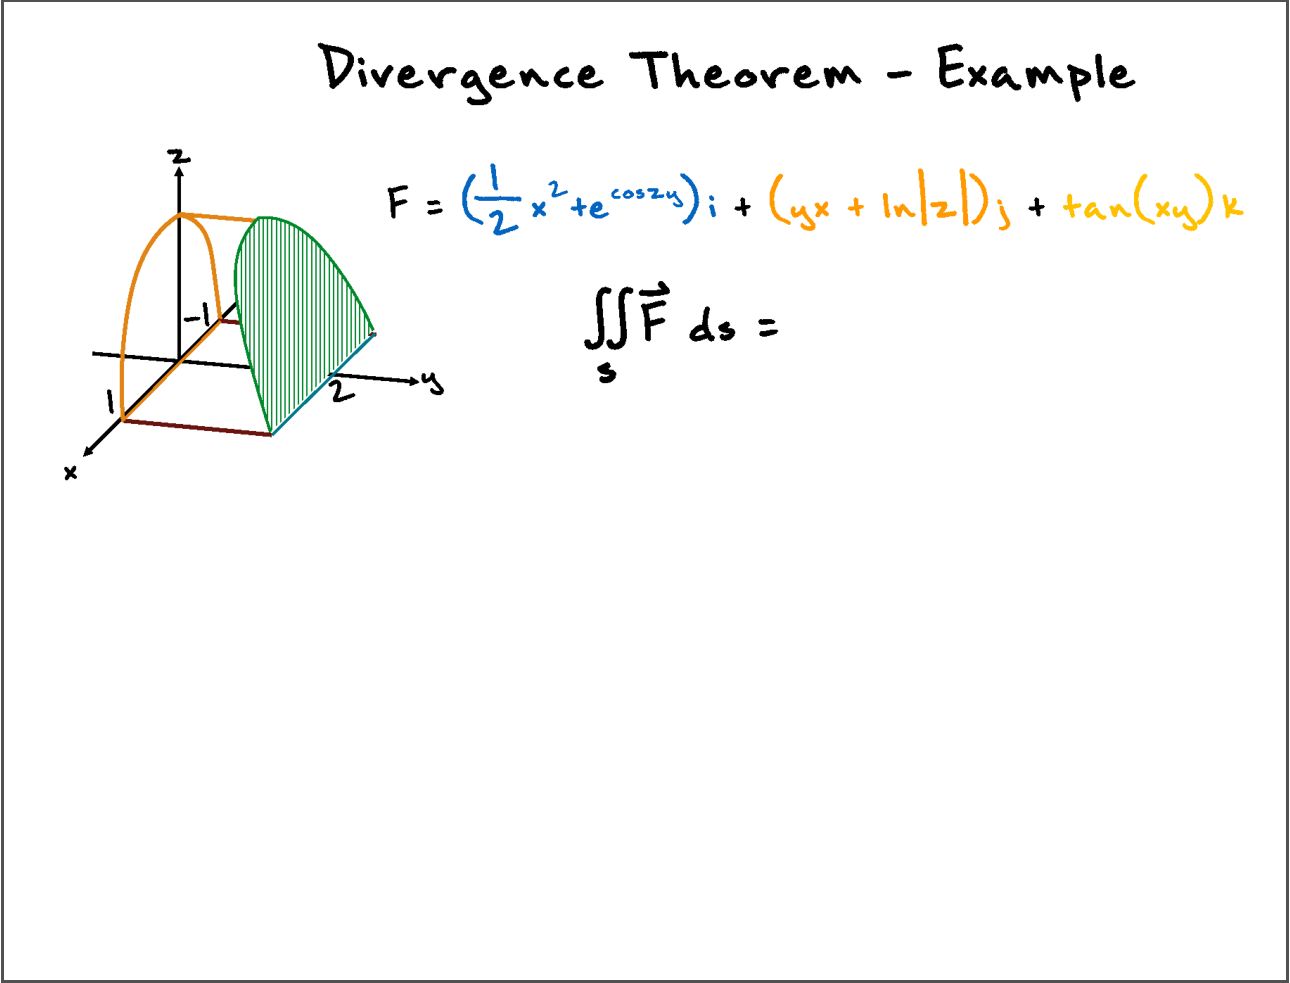
\includegraphics[width=1\columnwidth]{figures/videoslide1}
        \caption{Background (Audience View)}
    \end{subfigure}%
    ~ 
    \begin{subfigure}[t]{0.32\textwidth}
        \centering
        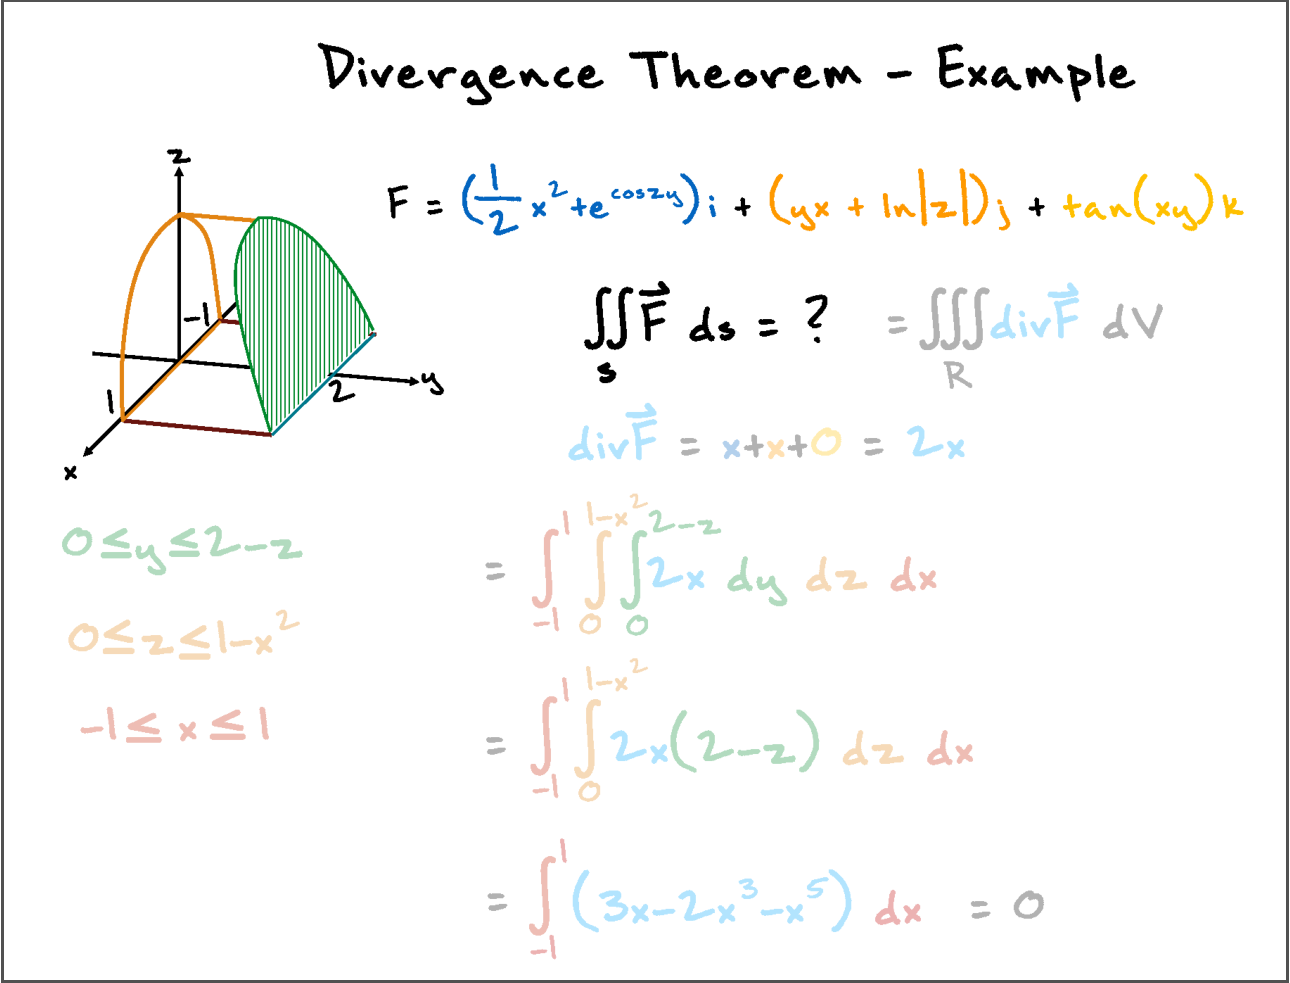
\includegraphics[width=1\columnwidth]{figures/videoslide2}
        \caption{Background + Foreground (Presenter View)}
    \end{subfigure}
    ~
        \begin{subfigure}[t]{0.32\textwidth}
        \centering
        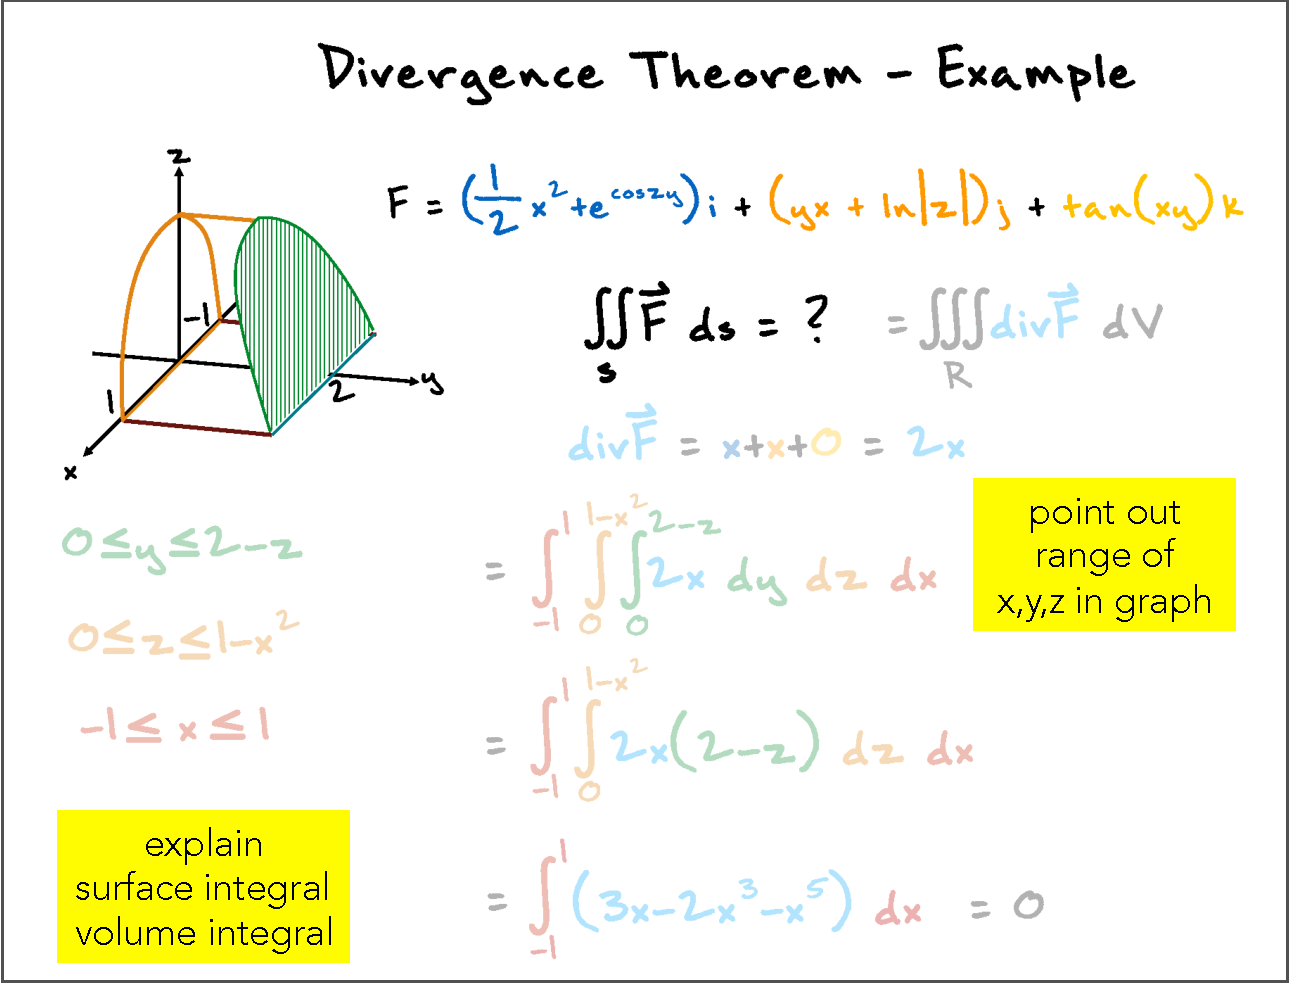
\includegraphics[width=1\columnwidth]{figures/videoslide3}
        \caption{Background + Foreground + Notes}
    \end{subfigure}
    \caption{Slide Layers in \interface. Slides are separated into foreground and background layers. \textbf{(a)} The background layer is always visible and it is what the audience sees initially. \textbf{(b)} The foreground layer is initially only visible on the presenter view, and is faded to distinguish it from the background. Presenters can reveal parts of it to the audience during delivery. The revealed parts appear on the audience view and becomes unfaded on the presenter view. \textbf{(c)} Optionally, presenters can also have the notes layer, which is only visible on the presenter view and acts as transparent speaker notes placed on top of the slides. }
    \label{fig:slidelayers}
\end{figure*}

\textbf{Pacing is important and context dependent.} 
The choice of tool also affects the pace of the presentation. Electronic slides are useful for displaying information quickly, which may explain why presenters prefer them for time-constrained settings. Inking takes time, but it allows presenters to have fine-grained control over the pace of the presentation. Depending on the subject matter, the pace of real time writing also makes it easier to follow for the audience. For example, when describing sequential processes like solving a math problem or explaining a complex diagram, both presenters and viewers find it more effective to write them out step-by-step in real-time. Slide animations can simulate this effect, but setting up fine-grained animations is tedious. As a result, animated presentations typically include a very coarse set of discrete steps. 

\textbf{Visual aesthetics matter but are difficult to achieve with inking.} Both as a presenter and as an audience, people frequently mentioned better visual aesthetics as an advantage of slides over inking. Presenters are often not satisfied with or even embarrassed by their own handwriting. They pointed out that it is even more difficult to write while talking at the same time. Even small operations, such as changing the pen color, seem burdensome during the lecture, as noted by Anderson\cite{anderson2004study}. 
% \wil{Previous two sentences don't seem to be about aesthetics. Is there a separate observation to make about timing? Or could this go into the first observation on context-dependent flexibility?}
%
From a viewing perspective, people like the legibility and organization that pre-authored slides provide. As \cite{frey2002learners} also mention, sometimes audiences even felt that lecturers are better organized when they present using electronic slides. 
%\wil{For the two points with citations, are these things that also came up in your interviews, or are you just citing previous findings? If the former, we should try to make that clear, as I did with the Anderson reference above.}

\section{Design Goals}

The above findings highlight the complementary attributes of electronic slides and inking. While slides are typically more organized and aesthetically pleasing, inking offers greater flexibility and fine-grained control at presentation time.
%
Our aim is to develop a presentation interface that combines the advantages of both existing technologies without increasing the burden on the presenter at authoring and presentation time.
%
More specifically, our system should achieve the following design goals. The first two goals are concerned with improving the presentation quality, while the last goal involves reducing the presenters' effort. 

\textbf{Maximize organization and aesthetics through pre-authored contents.} In order to improve presentation quality, we want to take full advantage of contents that presenters prepare beforehand. Pre-authored contents can help achieve visual aesthetics. It also \textit{forces} the presenter to organize the presentation ahead of time. 
 
\textbf{Maximize flexibility and fine-grained control during presentation delivery.} Presenters should have fine control over what visual content to present, and also when, how much, and how fast to present them. Moreover, these decisions need not be made ahead of time; instead, presenters should be able to implement and adjust them while delivering, according to the content and audience. 

\textbf{Minimize presenter effort during delivery as well as during preparation.} We want to give presenters more control, but without increasing their burden. Interactions during delivery should be as simple and natural as possible. Similarly, preparation itself should not take more effort than, for example, authoring regular slides. Moreover, presenters should be allowed to focus more on preparing the content itself rather than, for instance, spending time to setup animations effects for delivery. 

%These design goals are expressed in \interface in the following ways. 


